\documentclass[11pt]{amsart}
\usepackage{amsmath,amssymb,amsthm}
\usepackage[margin=1.1in]{geometry}
\usepackage{tikz}
\usepackage{hyperref}
\hypersetup{pdftitle={Toggling in w0(c) root order is conjugate to rowmotion: resolution of AIM Conjecture 3.2 and Thomas's conjecture},pdfauthor={Samson Fraser},pdfsubject={Mathematics - Combinatorics},pdfkeywords={AIM Conjecture 3.2, Thomas conjecture, dynamical algebraic combinatorics, rowmotion, toggles, birational rowmotion, Kreweras complement, Coxeter groups, root posets}}
\newtheorem{theorem}{Theorem}[section]
\newtheorem{lemma}[theorem]{Lemma}
\newtheorem{proposition}[theorem]{Proposition}
\newtheorem{corollary}[theorem]{Corollary}
\newtheorem{conjecture}[theorem]{Conjecture}
\theoremstyle{definition}
\newtheorem{definition}[theorem]{Definition}
\newtheorem{example}[theorem]{Example}
\newtheorem{remark}[theorem]{Remark}
\newcommand{\Tog}{\mathrm{Tog}}
\newcommand{\Row}{\mathrm{Row}}
\newcommand{\pr}{\prec_c}
\newcommand{\Hasse}{\mathcal H}

\title[Toggling in $w_0(c)$ root order]{Toggling in \texorpdfstring{$w_0(c)$}{w0(c)} root order is conjugate to rowmotion:\\ resolution of AIM Conjecture 3.2 and Thomas's conjecture}
\author{Samson Fraser}
\email{samsonmfraser@gmail.com}
\date{October 2026}
\begin{document}

\begin{abstract}
Toggling is a simple operation on a partially ordered set: it adds an element to a downward-closed subset, or removes one, whenever the result is still downward closed. Toggling every element in turn, from the top down, gives rowmotion, a map studied since the 1970s. Toggles also act on numerical labels, where they become rational maps, and there it is hard to tell whether a product of toggles ever returns to where it started. Even for rowmotion, this is known only for special posets.

In 2015, the problem list of the American Institute of Mathematics workshop on Dynamical Algebraic Combinatorics conjectured that one such product has order $2h$ on the root posets of types $A$, $B$, $H_3$ and $I_2(m)$, where $h$ is the Coxeter number. This product toggles the positive roots in an order determined by a Coxeter element. We resolve the conjecture. We prove that the product is conjugate to rowmotion in every finite crystallographic type and in types $H_3$ (for an explicit labelling of its roots) and $I_2(m)$; this also proves a 2013 conjecture of H.~Thomas. In the four types of the conjecture, it follows that the product returns to the identity after $2h$ steps. Its exact order is $2h$ in types $A_n$ ($n\ge2$) and $I_2(m)$ with $m$ odd, but only $h$ in types $B_n$, $H_3$ and $I_2(m)$ with $m$ even. The exceptional types and $H_3$ rely on exact computer calculations.
\end{abstract}
\maketitle

\section{Introduction}

\subsection{Toggles and rowmotion}
Let $P$ be a finite poset. For $v\in P$, the \emph{toggle} $t_v$ acts on order ideals of $P$ by adding $v$ to an ideal $I$ if $I\cup\{v\}$ is again an ideal, removing $v$ if $I\setminus\{v\}$ is again an ideal, and doing nothing otherwise. Each toggle is an involution, and $t_u$ and $t_v$ commute unless $u$ and $v$ are joined by an edge of the Hasse diagram. The group they generate is the \emph{toggle group} of $P$, introduced by Cameron and Fon-Der-Flaass~\cite{CFF} and developed systematically by Striker and Williams~\cite{SW}.

The most studied element of the toggle group is \emph{rowmotion}: toggling every element once, from the top of the poset to the bottom. As a map on antichains it goes back to Brouwer and Schrijver~\cite{BS}, and Cameron and Fon-Der-Flaass~\cite{CFF} showed that it is this product of toggles. For the root poset $\Phi^+$ of a finite Weyl group, Panyushev made three conjectures about rowmotion in its antichain form~\cite[Conj.~2.1]{Pan}:
\begin{itemize}
\item it has order $h$ if $w_0=-1$ and order $2h$ otherwise, where $h$ is the Coxeter number;
\item its $h$-th power is the involution induced by $-w_0$;
\item along every orbit, the average size of an antichain is $n/2$.
\end{itemize}
Armstrong, Stump and Thomas~\cite[Thm.~1.2]{AST} proved these conjectures by constructing a bijection, uniform in its definition, that carries rowmotion on antichains (nonnesting partitions) to the Kreweras complement on noncrossing partitions.

Einstein and Propp~\cite{EP} lifted toggles to the \emph{piecewise-linear} and \emph{birational} settings, in which a toggle becomes a rational map on labellings of $P$ (Section~\ref{sec:prelim}). Periodicity is much more delicate there. Grinberg and Roby~\cite{GR1,GR2} proved that birational rowmotion is periodic on products of two chains and on several triangles. They also showed that it can have infinite order, already on small graded posets such as the Boolean lattice $[2]^3$~\cite[\S20]{GR1}, and they report that it has infinite order on the root poset of type $D_4$~\cite[\S21]{GR1}. Musiker and Roby~\cite{MR} gave a lattice-path formula for its iterates on products of two chains. Okada~\cite{Oka} proved periodicity on all minuscule posets, and Johnson and Liu~\cite{JL} proved it on trapezoids, resolving a conjecture of Williams.

\subsection{Kreweras complements in the toggle group}
In his thesis~\cite[\S4.4.1]{Wil}, Williams records an observation of H.~Thomas. In type $A_n$, one of the toggle orders of Striker and Williams~\cite{SW} is the order of the roots given by the $c$-sorting word of $w_0$. Thomas proposed a model of the Kreweras complement inside the toggle group of the root poset~\cite[Def.~4.4.4]{Wil}, as follows. Fix a Coxeter element $c$, and let $\beta_1,\dots,\beta_N$ be the inversion sequence of the $c$-sorting word $w_0(c)$ of the longest element (Section~\ref{sec:prelim}). Toggling the elements of $\Phi^+$ in this order defines Thomas's \emph{nonnesting $c$-Kreweras complement}\footnote{This is a map on order ideals of $\Phi^+$, not the Kreweras complement $w\mapsto cw^{-1}$ on noncrossing partitions used in~\cite{AST}; this is why it is renamed $\mathrm{Krow}_c$ in~\cite{DFISTW}.}
\[\mathrm{Krew}_c=\Tog_{\beta_1\beta_2\cdots\beta_N}.\]
Thomas conjectured that these maps are all conjugate to rowmotion:

\begin{conjecture}[Thomas; {\cite[Conj.~4.4.5]{Wil}}]\label{conj:thomas}
For every finite Weyl group $W$, any two of the maps $\mathrm{Krew}_c$ are conjugate in the toggle group of $\Phi^+(W)$, and they are conjugate to rowmotion.
\end{conjecture}

In type $A$, Dequ\^ene, Frieden, Iraci, Schreier-Aigner, Thomas and Williams~\cite{DFISTW} constructed an explicit equivariant bijection between noncrossing partitions under the Kreweras complement and nonnesting partitions under the toggle product $\Tog_{\beta_1\cdots\beta_N}$. They call this product the Kroweras complement $\mathrm{Krow}_c$~\cite[Def.~4.2]{DFISTW}, and it is exactly the map $\mathrm{Krew}_c$ above. In particular $\mathrm{Krew}_c$ has order $2h$ in type $A$~\cite[Cor.~1.6]{DFISTW}. Their conjugation identity~\cite[Prop.~4.7]{DFISTW}, combined with the Striker--Williams conjugacy of promotion and rowmotion~\cite{SW}, yields Conjecture~\ref{conj:thomas} in type $A$. They also treated type $C$ by folding, at the level of equivariant bijections.

\subsection{The AIM problem}
The birational lift of $\mathrm{Krew}_c$ is the map $K_c$ obtained by toggling the root poset in the same order, using birational toggles. The problem list~\cite{AIM} of the 2015 AIM workshop on Dynamical Algebraic Combinatorics records the following.

\begin{quote}
Birational toggles in $w_0(c)$ root orders appear to continue to have order $2h$ in type $A_n$. This fails, for example, in type $D_4$ (as does birational rowmotion).

\textbf{Conjecture 3.2.} \emph{Birational toggles in $w_0(c)$ root orders have order $2h$ in the coincidental types $A$, $B$, $H_3$, $I_2(m)$.}
\end{quote}

Two features make this harder than the corresponding statement for rowmotion.

First, an inversion order of $w_0$ is in general not a linear extension of the root poset, so $K_c$ is not rowmotion, and the known periodicity results do not apply to it directly. The toggle order matters a great deal. On the four-element poset $[2]\times[2]$, rowmotion has order $4$, but $T_{(1,1)}\circ T_{(1,2)}\circ T_{(2,2)}\circ T_{(2,1)}$ has infinite order~\cite[Ex.~2.15]{GR1}, \cite{EP}.

Second, ``has order $2h$'' admits two readings: that $2h$ is the exact order, or that $2h$ is a period, i.e.\ $K_c^{2h}=\mathrm{id}$. The two readings already differ in rank two. The second is the form in which Armstrong, Stump and Thomas~\cite{AST} state Panyushev's conjecture. It is also the form of Hopkins' conjecture~\cite[Conj.~4.40]{Hop} that birational rowmotion on a coincidental root poset has order dividing $2h$. Panyushev's own formulation~\cite[Conj.~2.1]{Pan} specifies the exact order: $h$ if $w_0=-1$, and $2h$ otherwise.

\subsection{Results}
Our first result proves Thomas's conjecture in every finite crystallographic type, for the combinatorial and the birational toggle groups alike, and extends it to the noncrystallographic coincidental types.

\begin{theorem}\label{thm:conj}
Let $W$ be a finite Coxeter group of crystallographic type, or of type $H_3$ or $I_2(m)$ with Armstrong's root poset, labelled by roots as in Table~\ref{tab:H3} in type $H_3$. (In type $I_2(m)$ the labelling is irrelevant; see Section~\ref{sec:H3}.) Let $c$ be a Coxeter element. Then $\Tog_{\beta_1\cdots\beta_N}$ is conjugate to rowmotion in the toggle group of $\Phi^+(W)$, for combinatorial, piecewise-linear and birational toggles. In particular Conjecture~\ref{conj:thomas} holds.
\end{theorem}

Combining Theorem~\ref{thm:conj} with what is known about the order of birational rowmotion settles the AIM problem.

\begin{theorem}\label{thm:main}
Let $W$ be of type $A_n$, $B_n$ (with either the $B_n$ or the $C_n$ labelling of the root poset), $H_3$ (with the labelling of Table~\ref{tab:H3}) or $I_2(m)$, and let $c$ be any Coxeter element. Then $K_c^{2h}=\mathrm{id}$. The exact order of $K_c$ is:
\begin{itemize}
\item $2h=2(n+1)$ in type $A_n$ for $n\ge2$;
\item $h=2n$ in type $B_n$;
\item $h=10$ in type $H_3$;
\item $\mathrm{lcm}(2,m)$ in type $I_2(m)$, that is, $2h$ for $m$ odd and $h$ for $m$ even.
\end{itemize}
\end{theorem}

Thus Conjecture~3.2 holds when ``order $2h$'' is read as a period. Read literally, it is false: already for $B_2=I_2(4)$ the order is $4=h$. Since $w_0=-1$ exactly in types $B_n$, $H_3$ and $I_2(m)$ with $m$ even, the orders in Theorem~\ref{thm:main} follow Panyushev's dichotomy for combinatorial rowmotion.

Theorem~\ref{thm:conj} also explains the parenthetical remark in~\cite{AIM}. In type $D_4$ the map $K_c$ is conjugate to birational rowmotion, so the two maps have the same order, and by~\cite[\S21]{GR1} that order is infinite.

\subsection{Method}
A toggle order induces an acyclic orientation of the Hasse diagram, and reversing all edges at a source (a \emph{source-to-sink move}) amounts to conjugating by a single toggle. This principle goes back to the study of conjugacy of Coxeter elements~\cite{Shi,EE,MM}, and it is stated for toggle groups in~\cite[\S3]{EFGJMPR} (see also~\cite{DMR}). By a theorem of Pretzel~\cite{Pretzel}, two acyclic orientations are related by source-to-sink moves if and only if they have the same circulation around every cycle.

So it suffices to show that the orientation induced by $w_0(c)$ has circulation zero around every cycle, as does the orientation induced by rowmotion (Section~\ref{sec:orient}). Two classical facts about $c$-sorting words determine the orientation of every edge:
\begin{itemize}
\item Dyer's theory of reflection orders~\cite{Dyer} reduces the orientation of a cover $\gamma\lessdot\gamma+\alpha_s$ to the relative position of $\gamma$ and $\alpha_s$;
\item a compatibility property of Reading and Speyer~\cite{RS} expresses that position through the sign of a skew-symmetric form $\Omega_c$ (Section~\ref{sec:edges}).
\end{itemize}
Zero circulation then follows from a parallelism property of the small squares in the root poset, together with the fact that these squares generate all cycles (Sections~\ref{sec:squares} and~\ref{sec:all}). The exceptional types $E$, $F$, $G$ and the noncrystallographic type $H_3$ are finite checks (Sections~\ref{sec:all} and~\ref{sec:H3}). The orders are deduced in Section~\ref{sec:orders}.

\section{Preliminaries}\label{sec:prelim}

\subsection{Root posets}
Let $W$ be a finite Coxeter group with simple reflections $S=\{s_1,\dots,s_n\}$, simple roots $\Delta=\{\alpha_1,\dots,\alpha_n\}$, positive roots $\Phi^+$, $N=|\Phi^+|$, and Coxeter number $h$. For crystallographic $W$, the \emph{root poset} is $\Phi^+$ ordered by $\beta\le\beta'$ if and only if $\beta'-\beta$ is a nonnegative integer combination of simple roots. Its covers are exactly the relations $\gamma\lessdot\gamma+\alpha_s$ with $\gamma,\gamma+\alpha_s\in\Phi^+$, and it is graded by height. For $I_2(m)$ and $H_3$ we use Armstrong's root posets~\cite{Arm}, which Cuntz and Stump characterised as the unique posets with the expected enumerative properties~\cite{CS}; they are described in Section~\ref{sec:H3}. We write $\Hasse(P)$ for the Hasse diagram of a poset $P$, viewed as an undirected graph.

\subsection{\texorpdfstring{Coxeter elements and $c$-sorting words}{Coxeter elements and c-sorting words}}
A \emph{Coxeter element} is a product $c=s_{i_1}\cdots s_{i_n}$ of all simple reflections in some order; we fix such a reduced word. Consider the infinite word
\[c^\infty=s_{i_1}\cdots s_{i_n}s_{i_1}\cdots s_{i_n}\cdots.\]
Among its subwords that are reduced words for the longest element $w_0$, take the one whose sequence of positions is lexicographically first. This is the \emph{$c$-sorting word} $w_0(c)=a_1a_2\cdots a_N$. Its inversion sequence
\[\beta_k=s_{a_1}s_{a_2}\cdots s_{a_{k-1}}(\alpha_{a_k}),\qquad 1\le k\le N,\]
lists every positive root exactly once. We write $\beta\pr\beta'$ if $\beta$ occurs before $\beta'$ in this sequence.

\begin{example}\label{ex:A3}
Let $W=A_3$ and $c=s_1s_2s_3$. Then $w_0(c)=s_1s_2s_3\,s_1s_2\,s_1$, and the inversion sequence is
\[\alpha_1,\ \alpha_1+\alpha_2,\ \alpha_1+\alpha_2+\alpha_3,\ \alpha_2,\ \alpha_2+\alpha_3,\ \alpha_3 .\]
This is not a linear extension of the root poset: $\alpha_1+\alpha_2$ comes before $\alpha_2$.
\end{example}

\subsection{Toggles}
Let $\widehat P=P\sqcup\{\hat0,\hat1\}$, with $\hat0$ below and $\hat1$ above every element. A \emph{labelling} is a map $f:\widehat P\to\mathbb K$ to a field $\mathbb K$ (in practice a field of rational functions in the labels), with fixed boundary values $f(\hat0)=a$ and $f(\hat1)=b$. The \emph{birational toggle} at $v\in P$ is
\[(T_vf)(v)=\frac{\sum_{u\lessdot v}f(u)}{f(v)\sum_{u\gtrdot v}1/f(u)},\qquad (T_vf)(x)=f(x)\quad(x\neq v),\]
where the sums run over the lower and upper covers of $v$ in $\widehat P$~\cite{EP,GR1}. The piecewise-linear toggles are its tropicalisation~\cite{EP}. As in the combinatorial case, each $T_v$ is an involution, and $T_u$ and $T_v$ commute unless $u$ and $v$ are adjacent in $\Hasse(P)$~\cite[\S2]{GR1}. These two facts are all we use about toggles in Sections~\ref{sec:orient}--\ref{sec:all}, so those sections apply verbatim to combinatorial and piecewise-linear toggles.

For a total order $L=(x_1,\dots,x_N)$ of $P$ put
\[\Tog_L=T_{x_N}\circ\cdots\circ T_{x_2}\circ T_{x_1},\]
so that $x_1$ is toggled first. \emph{Birational rowmotion} is $\Row=\Tog_L$ for $L$ the reverse of a linear extension, so that higher elements are toggled first. We put
\[K_c=\Tog_{(\beta_1,\dots,\beta_N)}.\]
Thus $\mathrm{Krew}_c$, $\Tog_{\beta_1\cdots\beta_N}$ and $K_c$ denote the same word in the toggles, read in the combinatorial, a general, and the birational toggle group, respectively.

\section{Toggle orders, orientations and circulation}\label{sec:orient}
A total order $L$ of $P$ induces an acyclic orientation $O_L$ of $\Hasse(P)$: each edge points from the element toggled first to the element toggled later.

\begin{lemma}\label{lem:orient}
\begin{enumerate}
\item[(a)] $\Tog_L$ depends only on $O_L$. We write $\Tog_O:=\Tog_L$ for any total order $L$ with $O_L=O$.
\item[(b)] Let $x$ be a source of an acyclic orientation $O$, and let $O'$ be obtained from $O$ by reversing all edges at $x$, so that $x$ becomes a sink. Then $\Tog_{O'}=T_x\circ\Tog_{O}\circ T_x$.
\end{enumerate}
\end{lemma}

\begin{proof}
(a) The total orders inducing $O_L$ are the linear extensions of the partial order generated by $O_L$. Any two linear extensions of a poset are connected by a sequence of swaps of adjacent, incomparable elements. Two elements that are incomparable in this partial order are not joined by an edge of $\Hasse(P)$, so their toggles commute, and each swap leaves the product unchanged.

(b) Since $x$ is a source, by (a) we may choose a total order $L=(x_1,\dots,x_N)$ with $O_L=O$ and $x=x_1$. As $T_x$ is an involution,
\[T_x\circ\Tog_L\circ T_x=T_x\circ T_{x_N}\circ\cdots\circ T_{x_2},\]
which is $\Tog$ of the order $(x_2,\dots,x_N,x)$; this order induces $O'$.
\end{proof}

For a cycle $C$ of $\Hasse(P)$ with a chosen direction of traversal, the \emph{circulation} $\nu_C(O)$ of an orientation $O$ is the number of edges of $C$ oriented along the direction of traversal minus the number oriented against it. A source-to-sink move does not change any circulation: a cycle through $x$ uses two edges at $x$, one entering and one leaving $x$ in the direction of traversal, and reversing both swaps their contributions.

\begin{theorem}[Pretzel~\cite{Pretzel}; see also {\cite[Prop.~4.4]{DMR}}]\label{thm:pretzel}
Two acyclic orientations of a connected graph are related by a sequence of source-to-sink moves if and only if they have the same circulation around every cycle.
\end{theorem}

\begin{example}\label{ex:square}
On $[2]\times[2]$, the order $(2,1),(2,2),(1,2),(1,1)$ orients the unique $4$-cycle so that, traversed as $(1,1)\to(1,2)\to(2,2)\to(2,1)\to(1,1)$, three edges point against the direction of traversal and one along it. Its circulation is $-2$, whereas rowmotion's is $0$. So the two toggle products are not related by source-to-sink moves. Indeed, the first has infinite order and the second has order $4$~\cite[Ex.~2.15]{GR1}.
\end{example}

Call $g:P\to\mathbb Z$ a \emph{potential} for an orientation $O$ if $g(y)=g(x)+1$ for every edge $x\to y$ of $O$. Summing $g(\text{head})-g(\text{tail})$ around a cycle shows that an orientation with a potential has circulation $0$ around every cycle. Conversely, on a connected graph, zero circulation around every cycle allows one to define a potential by integrating along paths. The following corollary needs only the easy direction of Theorem~\ref{thm:pretzel}, and we include a short self-contained proof that also exhibits the conjugating element.

\begin{corollary}\label{cor:pot}
Let $P$ be a graded poset with connected Hasse diagram. If $O_L$ has circulation $0$ around every cycle (equivalently, admits a potential), then $\Tog_L$ is conjugate to $\Row$ in the toggle group. More precisely, there are $x_1,\dots,x_k\in P$ with $\Tog_L=T_{x_k}\cdots T_{x_1}\,\Row\,T_{x_1}\cdots T_{x_k}$.
\end{corollary}

\begin{proof}
Let $g$ be a potential for $O_L$. In the orientation induced by rowmotion every edge points from the higher to the lower element, so $\varphi=-\mathrm{rank}$ is a potential for it. Along every edge both $g$ and $\varphi$ change by $\pm1$, so $g-\varphi$ has constant parity on the connected graph $\Hasse(P)$. Adding a constant to $g$, which does not change $O_L$, we may assume that $g\ge\varphi$ and $g\equiv\varphi\pmod2$.

We modify $\varphi$ step by step. At each stage $\varphi$ is a potential for an acyclic orientation $O_\varphi$ (with $x\to y$ when $\varphi(y)=\varphi(x)+1$), and $\Tog_{O_\varphi}$ is conjugate to $\Row$ by a product of toggles. Suppose $\varphi\ne g$. Let $x$ minimise $\varphi$ on the set $U=\{v:\varphi(v)<g(v)\}$, so that $g(x)\ge\varphi(x)+2$. If a neighbour $y$ of $x$ had $\varphi(y)=\varphi(x)-1$, then $y\notin U$ by minimality, so $g(y)=\varphi(y)=\varphi(x)-1\le g(x)-3$, contradicting $|g(x)-g(y)|=1$. Hence every neighbour $y$ has $\varphi(y)=\varphi(x)+1$, so $x$ is a source of $O_\varphi$. Replacing $\varphi(x)$ by $\varphi(x)+2\le g(x)$ turns $x$ into a sink, and by Lemma~\ref{lem:orient}(b) it conjugates $\Tog_{O_\varphi}$ by $T_x$. Each step decreases $\sum_v(g-\varphi)(v)$ by $2$, so after finitely many steps $\varphi=g$, $O_\varphi=O_L$, and the claim follows.
\end{proof}

Since circulation is additive, it suffices to verify zero circulation on a set of cycles that spans the cycle space of $\Hasse(P)$ over $\mathbb Q$.

\begin{example}\label{ex:A3pot}
Figure~\ref{fig:A3} shows the orientation of Example~\ref{ex:A3}. The numbers in brackets form a potential, so $K_c$ is conjugate to rowmotion in type $A_3$ for this $c$.
\end{example}

\begin{figure}[h]\centering
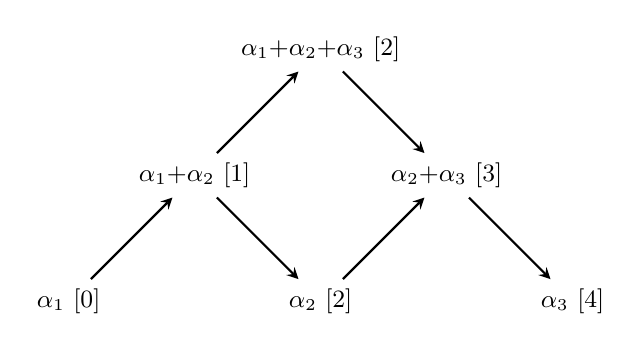
\begin{tikzpicture}[scale=1.6,>=stealth,every node/.style={font=\small}]
\node (a1) at (0,0) {$\alpha_1\ [0]$};
\node (a2) at (2,0) {$\alpha_2\ [2]$};
\node (a3) at (4,0) {$\alpha_3\ [4]$};
\node (a12) at (1,1) {$\alpha_1{+}\alpha_2\ [1]$};
\node (a23) at (3,1) {$\alpha_2{+}\alpha_3\ [3]$};
\node (a123) at (2,2) {$\alpha_1{+}\alpha_2{+}\alpha_3\ [2]$};
\draw[->,thick] (a1) -- (a12);
\draw[->,thick] (a12) -- (a2);
\draw[->,thick] (a2) -- (a23);
\draw[->,thick] (a23) -- (a3);
\draw[->,thick] (a12) -- (a123);
\draw[->,thick] (a123) -- (a23);
\end{tikzpicture}
\caption{The root poset of $A_3$ with the orientation induced by $w_0(c)$ for $c=s_1s_2s_3$ (each edge points away from the root toggled first) and a potential in brackets.}\label{fig:A3}
\end{figure}

\section{Orientation of cover edges}\label{sec:edges}
In this section $W$ is crystallographic. We determine the orientation of each edge $\gamma\lessdot\gamma+\alpha_s$ of $\Hasse(\Phi^+)$ in two steps.

\subsection{Reduction to a comparison with a simple root}
The order $\pr$ is a \emph{reflection order} in the sense of Dyer, since it is the inversion order of a reduced word for $w_0$.

\begin{lemma}[Dyer {\cite[(2.2), (2.13)]{Dyer}}]\label{lem:dyer}
If $\alpha\pr\gamma$ and $\beta=x\alpha+y\gamma\in\Phi^+$ with $x,y>0$, then $\alpha\pr\beta\pr\gamma$.
\end{lemma}

\begin{corollary}\label{cor:up}
For a cover $\gamma\lessdot\gamma+\alpha_s$, the edge is oriented upward (that is, $\gamma\pr\gamma+\alpha_s$) if and only if $\gamma\pr\alpha_s$.
\end{corollary}

\begin{proof}
The root $\gamma+\alpha_s$ is a positive combination of $\gamma$ and $\alpha_s$, so by Lemma~\ref{lem:dyer} it lies between them in $\pr$. If $\gamma\pr\alpha_s$, then $\gamma\pr\gamma+\alpha_s$; if $\alpha_s\pr\gamma$, then $\gamma+\alpha_s\pr\gamma$.
\end{proof}

\subsection{\texorpdfstring{The form $\Omega_c$}{The form Omega\_c}}
Let $(\cdot,\cdot)$ be a $W$-invariant inner product, let $a_{ij}$ be the Cartan matrix, and put $f_i=(\alpha_i,\alpha_i)/2$, so that $(\alpha_i,\alpha_j)=f_ia_{ij}$. Define a skew-symmetric bilinear form $\Omega_c$ on the root lattice by
\[\Omega_c(\alpha_i,\alpha_j)=\begin{cases}-(\alpha_i,\alpha_j)&\text{if $s_i$ precedes $s_j$ in $c$,}\\ \phantom{-}(\alpha_i,\alpha_j)&\text{if $s_j$ precedes $s_i$ in $c$,}\\ 0&\text{if $i=j$ or $a_{ij}=0$.}\end{cases}\]
It suffices to treat irreducible $W$. Then $\Omega_c$ is a positive scalar multiple of the form $\omega_c$ of Reading and Speyer~\cite{RS}, defined by $\omega_c(\alpha_i,\alpha_j)=-K(\alpha_i,\alpha_j)$ when $s_i$ precedes $s_j$, where $K(\alpha_i,\alpha_j)=\delta(i)a_{ij}$. Here $\delta(i)>0$ are the symmetrising constants of~\cite[\S2.2]{RS}, so that $\alpha_i^\vee=\delta(i)^{-1}\alpha_i$ and $K$ is symmetric. Since both $(\delta(i)a_{ij})$ and $(f_ia_{ij})$ are symmetric, we have $\delta(i)/\delta(j)=f_i/f_j$ whenever $a_{ij}\ne0$, so $\delta(i)/f_i$ is constant on an irreducible diagram. Note also that $\Omega_c$ depends only on $c$, not on the chosen reduced word.

\begin{lemma}[Reading--Speyer {\cite[Prop.~3.11]{RS}}; Reading {\cite[Cor.~4.4]{Rea}}]\label{lem:RS}
If $\beta\pr\beta'$, then $\Omega_c(\beta,\beta')\ge0$, with strict inequality unless the reflections $s_\beta$ and $s_{\beta'}$ commute.
\end{lemma}

Here Reading's theorem~\cite[Cor.~4.4]{Rea} that $w_0$ is $c$-sortable is what makes Reading--Speyer's Proposition~3.11 applicable to the inversion order of $w_0(c)$.

\begin{lemma}\label{lem:rule}
Let $\gamma\lessdot\gamma+\alpha_s$ be a cover with $\Omega_c(\gamma,\alpha_s)\neq0$. Then the edge is oriented upward if and only if $\Omega_c(\gamma,\alpha_s)>0$.
\end{lemma}

\begin{proof}
If the edge is oriented upward, then $\gamma\pr\alpha_s$ by Corollary~\ref{cor:up}, so $\Omega_c(\gamma,\alpha_s)\ge0$ by Lemma~\ref{lem:RS}. If it is oriented downward, then $\alpha_s\pr\gamma$, so $\Omega_c(\alpha_s,\gamma)\ge0$, that is, $\Omega_c(\gamma,\alpha_s)\le0$. Since $\Omega_c(\gamma,\alpha_s)\ne0$, its sign determines the orientation.
\end{proof}

Write $\gamma=\sum_t\gamma_t\alpha_t$ and $t\sim s$ for adjacency in the Dynkin diagram. Then
\begin{equation}\label{eq:omega}
\Omega_c(\gamma,\alpha_s)=\sum_{t\sim s}\sigma_{ts}\,(\alpha_t,\alpha_s)\,\gamma_t,\qquad \sigma_{ts}=\begin{cases}-1&\text{if $s_t$ precedes $s_s$ in $c$,}\\ +1&\text{if $s_s$ precedes $s_t$ in $c$.}\end{cases}
\end{equation}
In Example~\ref{ex:A3}, with $(\alpha_i,\alpha_i)=2$, we get $\Omega_c(\alpha_1,\alpha_2)=\Omega_c(\alpha_2,\alpha_3)=1$. So the edge $\alpha_1\lessdot\alpha_1+\alpha_2$ points up and the edge $\alpha_2\lessdot\alpha_1+\alpha_2$ points down, as in Figure~\ref{fig:A3}.

Whenever Lemma~\ref{lem:rule} applies to every cover, the orientation, and hence $K_c$, depends only on $c$ and not on the reduced word chosen for it. In types $F_4$, $G_2$ and $H_3$ we checked all reduced words directly.

\begin{lemma}\label{lem:nonzero}
$\Omega_c(\gamma,\alpha_s)\ne0$ for every cover $\gamma\lessdot\gamma+\alpha_s$ in types $A_n$, $B_n$, $D_n$ and $E_n$.
\end{lemma}

\begin{proof}
Simply laced types (normalise $(\alpha,\alpha)=2$ for all roots): since $\gamma$ and $\gamma+\alpha_s$ are both roots of norm $2$, we get $(\gamma,\alpha_s)=-1$. Expanding, $2\gamma_s-\sum_{t\sim s}\gamma_t=-1$, so $\sum_{t\sim s}\gamma_t$ is odd. By~\eqref{eq:omega}, $\Omega_c(\gamma,\alpha_s)=\sum_{t\sim s}\pm\gamma_t$ has the same parity, so it is nonzero.

Type $B_n$: take simple roots $\alpha_k=e_k-e_{k+1}$ ($k<n$) and $\alpha_n=e_n$, with $(e_i,e_j)=\delta_{ij}$, so that $(\alpha_k,\alpha_{k\pm1})=-1$. The covers are
\[e_i-e_j\lessdot e_i-e_{j+1},\quad e_i-e_n\lessdot e_i,\quad e_i-e_j\lessdot e_{i-1}-e_j,\quad e_i\lessdot e_{i-1},\quad e_i\lessdot e_i+e_n,\]
\[e_i+e_j\lessdot e_{i-1}+e_j,\qquad e_i+e_j\lessdot e_i+e_{j-1}\ (j-1>i).\]
In all but the last family, exactly one neighbour $t$ of $s$ has $\gamma_t\neq0$, and $\gamma_t=1$, so $|\Omega_c(\gamma,\alpha_s)|=1$. In the last family, $s=j-1$ has the neighbours $j-2$ and $j$, with coefficients $1$ and $2$ in $\gamma$, so $|\Omega_c(\gamma,\alpha_s)|\in\{1,3\}$.
\end{proof}

\section{Squares and the cycle space}\label{sec:squares}
A \emph{square} of $\Phi^+$ is a quadruple $(\gamma,\ \gamma+\alpha_s,\ \gamma+\alpha_t,\ \gamma+\alpha_s+\alpha_t)$ of positive roots with $s\neq t$. It is a $4$-cycle in $\Hasse(\Phi^+)$, consisting of two \emph{$s$-edges} and two \emph{$t$-edges}. We write it as $(\gamma;\ s,t)$.

\begin{lemma}\label{lem:square}
Suppose that $s$ and $t$ are not adjacent in the Dynkin diagram, and that $\Omega_c$ is nonzero on all four edges of the square $(\gamma;\ s,t)$. Then opposite edges of the square are parallel, and its circulation is $0$.
\end{lemma}

\begin{proof}
Since $\Omega_c(\alpha_t,\alpha_s)=0$, we have $\Omega_c(\gamma+\alpha_t,\alpha_s)=\Omega_c(\gamma,\alpha_s)$. By Lemma~\ref{lem:rule} the two $s$-edges are therefore both oriented upward or both downward, and likewise the two $t$-edges. Going around the square, the two $s$-edges are traversed in opposite directions, and so are the two $t$-edges, so the circulation is $0$.
\end{proof}

In simply laced types, no square has adjacent $s$ and $t$. Indeed, suppose $s\sim t$, so that $(\alpha_s,\alpha_t)=-1$. Since $\gamma\lessdot\gamma+\alpha_t$, the proof of Lemma~\ref{lem:nonzero} gives $(\gamma,\alpha_t)=-1$. Hence $(\gamma+\alpha_s,\alpha_t)=-2$, and
\[\|\gamma+\alpha_s+\alpha_t\|^2=\|\gamma+\alpha_s\|^2+2(\gamma+\alpha_s,\alpha_t)+\|\alpha_t\|^2=2-4+2=0,\]
which is impossible for a root. In type $B_n$, the list of covers in the proof of Lemma~\ref{lem:nonzero} shows that every square has one of the forms
\[(e_i-e_j;\ i-1,\,j),\quad (e_i-e_n;\ i-1,\,n),\quad (e_i;\ i-1,\,n),\quad (e_i+e_j;\ i-1,\,j-1)\ \ (j-1>i),\]
and in each, $s$ and $t$ are non-adjacent.

\begin{lemma}\label{lem:grid}
In types $A_n$ and $B_n$, the squares span the cycle space of $\Hasse(\Phi^+)$.
\end{lemma}

\begin{proof}
We embed $\Phi^+$ in the lattice $\mathbb Z^2$.

\emph{Type $A_n$.} Send $\alpha_i+\dots+\alpha_j$ to $(i,j)$. The image is the staircase $\Sigma_A=\{(i,j):1\le i\le j\le n\}$. The covers, which add $\alpha_{i-1}$ or $\alpha_{j+1}$, become exactly the unit steps $(i,j)\to(i-1,j)$ and $(i,j)\to(i,j+1)$ inside $\Sigma_A$.

\emph{Type $B_n$.} Send $e_i-e_j\mapsto(i,j)$, $e_i\mapsto(i,n+1)$ and $e_i+e_j\mapsto(i,2n+2-j)$. The image is $\Sigma_B=\{(i,p):1\le i\le n,\ i+1\le p\le 2n+1-i\}$, and each family of covers in the proof of Lemma~\ref{lem:nonzero} becomes a unit step inside $\Sigma_B$. Conversely, every unit step between two points of $\Sigma_B$ arises this way. A step $(i,p)\to(i-1,p)$ adds $\alpha_{i-1}$. A step $(i,p)\to(i,p+1)$ adds a simple root that depends only on $p$: it is $\alpha_p$ for $p<n$, $\alpha_n$ for $p\in\{n,n+1\}$, and $\alpha_{2n+1-p}$ for $p\ge n+2$.

In both cases $\Hasse(\Phi^+)$ is thereby identified with the \emph{induced} grid graph on $\Sigma$, whose edges are all unit steps between points of $\Sigma$. A unit square of the lattice has all four corners in $\Sigma$ if and only if it is the image of a square of $\Phi^+$. Each region $\Sigma$ is connected and both row-convex and column-convex.

Consider the plane drawing of this graph. We claim that every bounded face is a unit square. Suppose that a bounded face $F$ contains two adjacent open unit cells. The unit segment between them is not an edge of the graph, so at least one of its endpoints $q$ is not in $\Sigma$. This lattice point lies on no edge, so it belongs to $F$. Since $F$ is bounded, each horizontal ray from $q$ leaves $F$, so it meets the boundary of $F$. That boundary consists of edges between points of $\Sigma$, and it meets the horizontal line through $q$ only at points of $\Sigma$. So $\Sigma$ contains points on both sides of $q$ in its row, and row-convexity forces $q\in\Sigma$, a contradiction. Hence every bounded face is a single unit cell, whose boundary is the image of a square of $\Phi^+$. For a connected plane graph, the boundaries of the bounded faces span the cycle space, which proves the lemma.
\end{proof}

\begin{proposition}\label{prop:AB}
In types $A_n$ and $B_n$, $K_c$ is conjugate to $\Row$ for every Coxeter element $c$.
\end{proposition}

\begin{proof}
By Lemma~\ref{lem:nonzero}, $\Omega_c$ is nonzero on every cover. By the discussion after Lemma~\ref{lem:square}, every square has non-adjacent indices, so by Lemma~\ref{lem:square} every square has circulation $0$. By Lemma~\ref{lem:grid} the squares span the cycle space, so every cycle has circulation $0$, and Corollary~\ref{cor:pot} applies.
\end{proof}

\section{All crystallographic types}\label{sec:all}
\begin{theorem}\label{thm:thomas}
For every finite crystallographic Coxeter group $W$ and every Coxeter element $c$, the map $\Tog_{\beta_1\cdots\beta_N}$ is conjugate to rowmotion in the combinatorial, piecewise-linear and birational toggle groups of $\Phi^+(W)$. In particular Conjecture~\ref{conj:thomas} holds.
\end{theorem}

\begin{proof}
It suffices to treat irreducible $W$. As in Proposition~\ref{prop:AB}, it suffices to show that the squares span the cycle space of $\Hasse(\Phi^+)$ and that every square has circulation $0$. Types $A_n$ and $B_n$ are Proposition~\ref{prop:AB}. Homology is taken with $\mathbb Q$ coefficients.

\emph{Type $D_n$ ($n\ge4$).} Take simple roots $\alpha_k=e_k-e_{k+1}$ ($k<n$) and $\alpha_n=e_{n-1}+e_n$. The map $e_i-e_j\mapsto(i,j)$, $e_i+e_j\mapsto(i,2n-j)$ sends $\Phi^+$ onto the region
\[\Sigma=\{(i,p):1\le i\le n-1,\ i+1\le p\le 2n-1-i\}.\]
It is injective except that $e_i-e_n$ and $e_i+e_n$ both go to $(i,n)$. Accordingly, $\Hasse(\Phi^+)$ is the grid graph of $\Sigma$ with the column $p=n$ doubled into two columns $n^-$ and $n^+$, each joined to the columns $n-1$ and $n+1$.

Let $X^\pm$ be the square complex on $\Sigma$ that uses the column $n^\pm$. Each is the induced grid complex of a row- and column-convex region, so by the argument of Lemma~\ref{lem:grid} its unit squares span its cycle space, i.e.\ $H_1(X^\pm)=0$. The unit squares of $X^\pm$ are squares of $\Phi^+$, and the $1$-skeleton of $X^-\cup X^+$ is $\Hasse(\Phi^+)$. The intersection $X^-\cap X^+$ consists of two connected, contractible pieces, $p\le n-1$ and $p\ge n+1$. By the Mayer--Vietoris sequence, $H_1(X^-\cup X^+)$ is one-dimensional, generated by a cycle through $(i,n-1),(i,n^-),(i,n+1),(i,n^+)$. This cycle is the boundary of the square $(e_i-e_{n-1};\ n-1,\,n)$. Hence the squares span the cycle space. Since $D_n$ is simply laced, Lemmas~\ref{lem:nonzero} and~\ref{lem:square} apply to every square.

\emph{Type $C_n$.} Take $\alpha_k=e_k-e_{k+1}$ ($k<n$) and $\alpha_n=2e_n$, with $(e_i,e_j)=\delta_{ij}$, so that $(\alpha_k,\alpha_{k+1})=-1$ for $k\le n-2$ and $(\alpha_{n-1},\alpha_n)=-2$. The covers are
\[e_i-e_j\lessdot e_i-e_{j+1},\quad e_i-e_n\lessdot e_i+e_n,\quad e_i-e_j\lessdot e_{i-1}-e_j,\quad e_i+e_j\lessdot e_{i-1}+e_j,\]
\[e_i+e_j\lessdot e_i+e_{j-1}\ (j-1>i),\qquad e_i+e_{i+1}\lessdot 2e_i,\qquad 2e_i\lessdot e_{i-1}+e_i .\]
The map $e_i-e_j\mapsto(i,j)$, $e_i+e_j\mapsto(i,2n+1-j)$, $2e_i\mapsto(i,2n+1-i)$ identifies $\Hasse(\Phi^+(C_n))$ with the induced grid graph on the region $\Sigma_B$ of Lemma~\ref{lem:grid}, so the squares span the cycle space by the same argument.

On each cover above, the nonzero contributions $|(\alpha_u,\alpha_s)|\gamma_u$ ($u\sim s$) in~\eqref{eq:omega} form one of the multisets $\{1\}$, $\{2\}$ or $\{1,2\}$. Hence $\Omega_c(\gamma,\alpha_s)\in\{\pm1,\pm2,\pm3\}$ is nonzero, and Lemma~\ref{lem:rule} applies.

Squares with non-adjacent $s,t$ are handled by Lemma~\ref{lem:square}. The squares with adjacent $s,t$ are exactly $(e_k+e_{k+1};\ k-1,\,k)$.
\begin{itemize}
\item For the two $s$-edges, $\Omega_c(\gamma,\alpha_s)$ and $\Omega_c(\gamma+\alpha_t,\alpha_s)$ both come from the single neighbour $k$, with coefficients $1$ and $2$, so they have the same sign.
\item For the two $t$-edges, $|\Omega_c(\gamma,\alpha_t)|=2$ and $|\Omega_c(\alpha_s,\alpha_t)|=1$, so adding $\alpha_s$ to $\gamma$ does not change the sign.
\end{itemize}
Hence these squares also have parallel opposite edges and circulation $0$.

\emph{Types $E_6,E_7,E_8,F_4,G_2$.} These are finitely many cases. For every ordering of $S$ we computed $w_0(c)$ and the induced orientation, and verified in exact integer arithmetic that it admits a potential. There are $720$, $5040$, $40320$, $24$ and $2$ orderings respectively, and every one admits a potential. This suffices by Corollary~\ref{cor:pot}. As an independent check, we computed the rank of the square cycles modulo the prime $2^{31}-1$. Full rank modulo a prime implies full rank over $\mathbb Q$, so this confirms that in these types too the squares span the cycle space. We also checked that every square has parallel opposite edges.
\end{proof}

\begin{remark}\label{rem:other}
Independently of the proofs above, the existence of a potential was verified by computer for every ordering of $S$ in types $A_n$ ($n\le9$) and $B_n$, $C_n$, $D_n$ ($n\le8$).
\end{remark}

\begin{remark}\label{rem:comb}
Combining Theorem~\ref{thm:thomas} with the theorem of Armstrong, Stump and Thomas~\cite[Thm.~1.2]{AST}, the combinatorial map $\mathrm{Krew}_c$ has order $h$ if $w_0=-1$ and $2h$ otherwise, for every finite Weyl group and every Coxeter element $c$. This extends~\cite[Cor.~1.6]{DFISTW} beyond type $A$. Moreover $\mathrm{Krew}_c$ has the same orbit structure as rowmotion, hence as the Kreweras complement on noncrossing partitions~\cite{AST}, so an equivariant bijection between the two actions exists in every type.
\end{remark}

\section{The noncrystallographic types}\label{sec:H3}

\subsection{\texorpdfstring{Type $I_2(m)$}{Type I2(m)}}
Armstrong's root poset of $I_2(m)$ is $\{x,y\}\oplus(z_1<\dots<z_{m-2})$: two incomparable minimal elements below a chain. Its Hasse diagram is a tree, so it has no cycles. By Corollary~\ref{cor:pot}, every toggle order of it is conjugate to $\Row$. In particular, $K_c$ is conjugate to $\Row$ whatever labelling of the poset by roots of $I_2(m)$ is used. It remains to find the order of $\Row$.

Write $f'$ for the labelling after the toggles performed so far. Rowmotion toggles $z_{m-2},\dots,z_1$, and then $x$ and $y$. When $x$ and $y$ are toggled, they receive the new labels $D/(Uf(x))$ and $D/(Uf(y))$, where $D=f(\hat0)$ and $U=1/f'(z_1)$ are the same for both. Hence $r=f(x)/f(y)$ is mapped to $1/r$. Put $\Sigma_{xy}=f(x)+f(y)$ and $\Sigma^*_{xy}=1/f(x)+1/f(y)$. Then the new values are $(D/U)\,\Sigma^*_{xy}$ and $(U/D)\,\Sigma_{xy}$, so $k=\Sigma_{xy}\Sigma^*_{xy}=(1+r)^2/r$ is invariant, and $\Sigma_{xy}$ is mapped to $kD/(U\Sigma_{xy})$.

Comparing with the toggle rule shows that $(\Sigma_{xy},z_1,\dots,z_{m-2})$ evolves exactly as birational rowmotion on a chain of $m-1$ elements whose bottom label is $kD$. That map has exact order $m$: a chain of $m-1$ elements is $(m-1)$-graded, so this follows from~\cite[Prop.~7.3]{GR1}. Since $f(x)$ and $f(y)$ are recovered from $r$ and $\Sigma_{xy}$, and $r\mapsto1/r$ has period $2$, the order of $\Row$ on $I_2(m)$ is $\mathrm{lcm}(2,m)$.

\subsection{\texorpdfstring{Type $H_3$}{Type H3}}
We use the simple roots of $H_3$ with $m(s_1,s_2)=5$ and $m(s_2,s_3)=3$, and put $\tau=(1+\sqrt5)/2$. In~\cite[\S3.2, Fig.~2]{CS} the $30$ positive roots of $D_6$, written in an orthonormal basis $v_1,\dots,v_6$, are grouped into $15$ pairs, one for each positive root of $H_3$. From each pair take the vector that is lexicographically greater in the coordinates $v_1,\dots,v_6$, and order these $15$ roots by the root order of $D_6$. The result is Armstrong's $H_3$ root poset: it has $32=\mathrm{Cat}(H_3)$ order ideals and rank sizes $3,2,2,2,2,1,1,1,1$.

Each element is labelled by the $H_3$ root it represents. For a $D_6$ root $a=(a_1,\dots,a_6)$ in simple-root coordinates, the vector $(a_5+\tau a_3,\ a_2+\tau a_4,\ a_1+\tau a_6)$ is $1$ or $\tau$ times a unique positive root of $H_3$ in simple-root coordinates, and that root is the label of $a$. Table~\ref{tab:H3} lists the result. As Williams notes, for $H_3$ the labelling is part of the data of the problem. In this poset covers are not in general of the form $\beta\lessdot\beta+\alpha_s$ (for example $(1,0,0)\lessdot(\tau,1,0)$), so Sections~\ref{sec:edges} and~\ref{sec:squares} do not apply, and we argue by computer.

\begin{table}[h]\centering\small
\begin{tabular}{ccc|ccc|ccc}
$D_6$ root & & $H_3$ root & $D_6$ root & & $H_3$ root & $D_6$ root & & $H_3$ root\\\hline
$100000$&$\mapsto$&$(0,0,1)$ & $011000$&$\mapsto$&$(\tau,1,0)$ & $111101$&$\mapsto$&$(1,\tau,\tau)$\\
$010000$&$\mapsto$&$(0,1,0)$ & $111000$&$\mapsto$&$(\tau,1,1)$ & $111111$&$\mapsto$&$(\tau,\tau,\tau)$\\
$110000$&$\mapsto$&$(0,1,1)$ & $011100$&$\mapsto$&$(1,\tau,0)$ & $111211$&$\mapsto$&$(\tau,\tau+1,\tau)$\\
$001000$&$\mapsto$&$(1,0,0)$ & $011110$&$\mapsto$&$(\tau,\tau,0)$ & $112211$&$\mapsto$&$(\tau+1,\tau+1,\tau)$\\
 & & & $111100$&$\mapsto$&$(\tau,\tau+1,1)$ & $122211$&$\mapsto$&$(\tau+1,2\tau,\tau)$\\
 & & & $111110$&$\mapsto$&$(\tau+1,\tau+1,1)$ & & & \\
\end{tabular}
\caption{The $H_3$ root poset inside $\Phi^+(D_6)$ ($D_6$ roots in simple-root coordinates) and its labelling by positive roots of $H_3$ (simple-root coordinates).}\label{tab:H3}
\end{table}

\emph{Conjugacy.} There are six orderings of $S$, giving four Coxeter elements up to commutation. For each, the orientation induced by $w_0(c)$ has circulation $0$ around every cycle of a cycle basis, so $K_c$ is conjugate to $\Row$ by Corollary~\ref{cor:pot}.

\emph{Periodicity.} Grinberg and Roby report a Sage computation showing $\Row^{10}=\mathrm{id}$ on this poset~\cite[\S21]{GR1}. We verified this deterministically. Let $x=(x_1,\dots,x_{15})$ be the generic labelling, with boundary labels $1$. We computed $F=\Row^5(x)$ and $G=\Row^{-5}(x)$ exactly, as reduced fractions in $\mathbb Z[x_1,\dots,x_{15}]$, using multivariate arithmetic with gcd normalisation; the largest polynomial has $11247$ terms. The result is $F=G$ identically, so $\Row^{10}=\mathrm{id}$ as rational maps. General boundary labels reduce to $(1,1)$ by the rescalings $f\mapsto\lambda f$ and $f(v)\mapsto t^{\mathrm{rank}(v)}f(v)$, which commute with all toggles. The same computation gives $\Row^5\neq\mathrm{id}$, and $\Row^2\neq\mathrm{id}$ at an explicit rational point, so the order is exactly $10=h$. An independent randomised identity test modulo four large primes agrees.

\section{\texorpdfstring{Orders of rowmotion and the proof of Theorem~\ref{thm:main}}{Orders of rowmotion and the proof of the main theorem}}\label{sec:orders}
By Theorem~\ref{thm:thomas} and Section~\ref{sec:H3}, $K_c$ is conjugate to $\Row$, so the two maps have the same order. It remains to recall the order of birational rowmotion on each root poset.

\emph{Type $A_n$.} The root poset $\Phi^+(A_n)$ is the triangle $\Delta(n+1)$ of Grinberg and Roby~\cite[Rem.~18.3]{GR2}, on which $\Row$ has order exactly $2(n+1)=2h$ for $n\ge2$~\cite[Cor.~18.9]{GR2}.

\emph{Type $B_n$.} The root poset $\Phi^+(B_n)$ is isomorphic to the triangle $\mathrm{NEtri}(2n)$~\cite[Rem.~19.3]{GR2}, for which Grinberg and Roby conjectured that $\Row$ has order $2n$~\cite[Conj.~19.5]{GR2}. This follows from the work of Johnson and Liu~\cite[Cor.~5.3]{JL} on the trapezoid
\[T_{r,s}=\{(I,J)\in[r+s-1]\times[s]: I-J<r,\ I+J>s\}\]
(with the product order), on which they show that rowmotion has order exactly $r+s$. The map $(i,p)\mapsto(p-1,n+1-i)$ is an isomorphism from the grid model of $\Phi^+(B_n)$ in Lemma~\ref{lem:grid} onto $T_{n,n}$, since it sends up-steps to unit steps. Johnson and Liu state their result for positive real labellings with boundary labels $1$. For graded posets, general boundary labels reduce to this case by renormalisation~\cite{EP}, and since $\mathbb R_{>0}^N$ is Zariski dense, $\Row^{2n}=\mathrm{id}$ holds as an identity of rational maps. So the order on $\Phi^+(B_n)$ is exactly $2n=h$. The type $C_n$ labelling gives an isomorphic poset.

\emph{Type $I_2(m)$.} The order is $\mathrm{lcm}(2,m)$ by Section~\ref{sec:H3}. This also follows from~\cite[Prop.~7.3]{GR1}, as noted in~\cite[\S21]{GR1}.

\emph{Type $H_3$.} The order is $10=h$ by Section~\ref{sec:H3}.

In each coincidental type the order divides $2h$. This proves $K_c^{2h}=\mathrm{id}$ and Theorem~\ref{thm:main}. As a sanity check, floating-point iteration of birational rowmotion at a random positive labelling recovers these orders for $A_n$ ($n\le5$), $B_n$ ($n\le6$) and $I_2(m)$ ($3\le m\le14$).

\begin{remark}[Hopkins' conjecture]\label{rem:hopkins}
Hopkins conjectured that birational rowmotion on every root poset of coincidental type has order dividing $2h$~\cite[Conj.~4.40]{Hop}. He noted that Grinberg and Roby had established it for $A_n$, $H_3$ and $I_2(m)$ (for $H_3$ by a computer calculation~\cite[\S21]{GR1}), leaving type $B_n$ open. As recently as 2023 Grinberg and Roby still described periodicity on all coincidental root posets as open~\cite{GR3}. The results recalled above settle it. The $B_n$ case is due to Johnson and Liu~\cite{JL}, via the isomorphism $\Phi^+(B_n)\cong T_{n,n}$. Our contribution is a deterministic exact certificate in type $H_3$.
\end{remark}

\section{Concluding remarks}\label{sec:remarks}

\begin{remark}[Related work]\label{rem:related}
The conjugacy of products of involutions whose orders differ by source-to-sink moves is classical for Coxeter elements~\cite{Shi,EE,MM}, and for toggle groups it appears in~\cite[\S3]{EFGJMPR}, where toggle actions on noncrossing partitions and their homomesies are also studied. For minuscule posets, Okada~\cite{Oka} proved that birational Coxeter-motion is periodic and conjugate to rowmotion. Thomas and Williams~\cite{TW} developed rowmotion as a sequence of local moves (``slow motion'') on trim lattices. What is new here is a uniform description of the toric-equivalence class, in the sense of~\cite{DMR}, of the $w_0(c)$ orientation, through the sign of $\Omega_c$.
\end{remark}

\begin{remark}[Open questions]
(1) Our proof in types $E$, $F$, $G$ and $H_3$ is computational. A uniform argument would be desirable, for instance one that extends the square analysis of Section~\ref{sec:squares} to the exceptional root posets and to Armstrong's noncrystallographic posets. (2) In type $H_3$, $K_c$ depends on the chosen labelling of the root poset by roots. It would be interesting to know which labellings give a map conjugate to rowmotion.
\end{remark}

\section*{Code}
All computations are in the ancillary files of this arXiv submission (Python and C++). The file \texttt{anc/README.md} lists, for each computational claim in the paper, the file, the command and the expected output. The files cover:
\begin{itemize}
\item the root posets, $c$-sorting words and orientations (\texttt{roots.py}, \texttt{orient.py});
\item the exact potential and square checks (\texttt{fastcheck.cpp}, \texttt{squares.cpp}, \texttt{omega.cpp});
\item the $H_3$ conjugacy check (\texttt{h3run.py});
\item the $H_3$ certificate (\texttt{h3\_sym\_half.py}, with its run log);
\item the floating-point sanity checks (\texttt{roworder.py}, \texttt{i2m.py}).
\end{itemize}

\section*{Use of AI}
I used Claude Opus 5.5 (Anthropic) throughout this project: to search the literature, to develop and test the arguments, to write and run the code, and to draft the text. I then had every part checked by separate Claude sessions acting as referees. They re-derived each proof, compared each cited statement with its source, and recomputed the computational claims, in part with code written from scratch. Their reports led to corrections that are included here. These checks were made with the same AI system and do not replace expert refereeing. Every computational claim can be reproduced from the ancillary files. The one statement that rests on a long computation, $\Row^{10}=\mathrm{id}$ in type $H_3$, is certified by an exact symbolic calculation, not a numerical one. I have read the final manuscript and take full responsibility for its contents; any remaining errors are mine.

\begin{thebibliography}{99}
\bibitem{Arm} D.~Armstrong, Generalized noncrossing partitions and combinatorics of Coxeter groups, Mem.\ Amer.\ Math.\ Soc.\ 202 (2009), no.~949.
\bibitem{AST} D.~Armstrong, C.~Stump, H.~Thomas, A uniform bijection between nonnesting and noncrossing partitions, Trans.\ Amer.\ Math.\ Soc.\ 365 (2013), 4121--4151; arXiv:1101.1277.
\bibitem{BS} A.~E.~Brouwer, A.~Schrijver, On the period of an operator, defined on antichains, Math.\ Centrum report ZW 24/74, Amsterdam, 1974.
\bibitem{CFF} P.~J.~Cameron, D.~G.~Fon-Der-Flaass, Orbits of antichains revisited, European J.\ Combin.\ 16 (1995), 545--554.
\bibitem{CS} M.~Cuntz, C.~Stump, On root posets for noncrystallographic root systems, Math.\ Comp.\ 84 (2015), 485--503; arXiv:1212.2876.
\bibitem{DFISTW} B.~Dequ\^ene, G.~Frieden, A.~Iraci, F.~Schreier-Aigner, H.~Thomas, N.~Williams, Charmed roots and the Kroweras complement, J.\ Lond.\ Math.\ Soc.\ (2) 110 (2024), no.~5, e70025; arXiv:2212.14831.
\bibitem{DMR} M.~Develin, M.~Macauley, V.~Reiner, Toric partial orders, Trans.\ Amer.\ Math.\ Soc.\ 368 (2016), no.~4, 2263--2287; arXiv:1211.4247.
\bibitem{Dyer} M.~Dyer, Hecke algebras and shellings of Bruhat intervals, Compositio Math.\ 89 (1993), 91--115.
\bibitem{EFGJMPR} D.~Einstein, M.~Farber, E.~Gunawan, M.~Joseph, M.~Macauley, J.~Propp, S.~Rubinstein-Salzedo, Noncrossing partitions, toggles, and homomesies, Electron.\ J.\ Combin.\ 23(3) (2016), P3.52; arXiv:1510.06362.
\bibitem{EP} D.~Einstein, J.~Propp, Combinatorial, piecewise-linear, and birational homomesy for products of two chains, Algebr.\ Comb.\ 4 (2021), no.~2, 201--224.
\bibitem{EE} H.~Eriksson, K.~Eriksson, Conjugacy of Coxeter elements, Electron.\ J.\ Combin.\ 16(2) (2009), R4.
\bibitem{GR1} D.~Grinberg, T.~Roby, Iterative properties of birational rowmotion, arXiv:1402.6178 (unabridged version~8; section numbers refer to this version); part~I published in Electron.\ J.\ Combin.\ 23(1) (2016), P1.33.
\bibitem{GR2} D.~Grinberg, T.~Roby, Iterative properties of birational rowmotion II: rectangles and triangles, Electron.\ J.\ Combin.\ 22(3) (2015), P3.40 (numbering as in arXiv:1402.6178).
\bibitem{GR3} D.~Grinberg, T.~Roby, Birational rowmotion over noncommutative rings, S\'em.\ Lothar.\ Combin.\ 89B (2023), Art.~50 (FPSAC 2023).
\bibitem{Hop} S.~Hopkins, Minuscule doppelg\"angers, the coincidental down-degree expectations property, and rowmotion, Exp.\ Math.\ 31 (2022), no.~3; arXiv:1902.07301.
\bibitem{JL} J.~Johnson, R.~I.~Liu, Plane partitions and rowmotion on rectangular and trapezoidal posets, S\'em.\ Lothar.\ Combin.\ 91B (2024), Art.~58 (FPSAC 2024); arXiv:2311.07133.
\bibitem{MM} M.~Macauley, H.~S.~Mortveit, On enumeration of conjugacy classes of Coxeter elements, Proc.\ Amer.\ Math.\ Soc.\ 136 (2008), no.~12, 4157--4165.
\bibitem{MR} G.~Musiker, T.~Roby, Paths to understanding birational rowmotion on products of two chains, Algebr.\ Comb.\ 2 (2019), no.~2, 275--304; arXiv:1801.03877.
\bibitem{Oka} S.~Okada, Birational rowmotion and Coxeter-motion on minuscule posets, Electron.\ J.\ Combin.\ 28 (2021), P1.17; arXiv:2004.05364.
\bibitem{Pan} D.~I.~Panyushev, On orbits of antichains of positive roots, European J.\ Combin.\ 30 (2009), 586--594.
\bibitem{AIM} J.~Propp, T.~Roby, J.~Striker, N.~Williams, Problems for 2015 AIM workshop on Dynamical Algebraic Combinatorics (May 29, 2015), \S3.2, \url{https://aimath.org/pastworkshops/dac_preworkshop.pdf}.
\bibitem{Pretzel} O.~Pretzel, On reorienting graphs by pushing down maximal vertices, Order 3 (1986), 135--153.
\bibitem{Rea} N.~Reading, Clusters, Coxeter-sortable elements and noncrossing partitions, Trans.\ Amer.\ Math.\ Soc.\ 359 (2007), no.~12, 5931--5958; arXiv:math/0507186.
\bibitem{RS} N.~Reading, D.~E.~Speyer, Sortable elements in infinite Coxeter groups, Trans.\ Amer.\ Math.\ Soc.\ 363 (2011), 699--761; arXiv:0803.2722.
\bibitem{Shi} J.-Y.~Shi, Conjugacy relation on Coxeter elements, Adv.\ Math.\ 161 (2001), 1--19.
\bibitem{SW} J.~Striker, N.~Williams, Promotion and rowmotion, European J.\ Combin.\ 33 (2012), 1919--1942; arXiv:1108.1172.
\bibitem{TW} H.~Thomas, N.~Williams, Rowmotion in slow motion, Proc.\ Lond.\ Math.\ Soc.\ (3) 119 (2019), no.~5, 1149--1178; arXiv:1712.10123.
\bibitem{Wil} N.~Williams, Cataland, Ph.D.\ thesis, University of Minnesota, 2013, \url{https://conservancy.umn.edu/items/a039fb17-102c-493e-a49f-bac8d0c92e20}.
\end{thebibliography}
\end{document}
